% En esta sección se presenta una breve descripción de la solución que se propone, 
% el principal objetivo de esta sección es poder dar el bosquejo de la solución 
% para que pueda ser evaluado. No es necesario detalles, pero sí mencionar sus 
% componentes generales. 
% Si las tecnologías que se van a utilizar ya están establecidas, se deberán 
% incluir aquí. De no estar definidas todas, enumerar las que sí están definidas 
% y explicar qué consideraciones tendrán en cuenta para definir las restantes.

\noindent Como respuesta a las problemáticas presentadas anteriormente nosotros desarrollamos una arquitectura
completamente distribuida, opuesta totalmente al modelo monolítico prevaleciente en la industria de los videojuegos. 
El estado del juego no se encuentra restringido a un único nodo servidor, sino que se encuentra 
distribuido en varios, cada uno con igual importancia y responsabilidades que el resto. El conjunto del estado en cada uno de estos nodos compone el 
estado del juego en su totalidad.

El aspecto central del videojuego desarrollado es el uso que hace del \textbf{modelo de actores}.
Dicho modelo se basa en el \textbf{actor} como mínima unidad de cómputo y el pasaje de \textbf{mensajes} como única manera
de compartir información entre los actores. En la práctica, esto significa que toda la lógica del juego
es procesada por los actores, y la comunicación entre ellos se realiza únicamente mediante mensajes.
Este paradigma, ideado por Carl Hewitt en los años 70, eliminá varios de los problemas presentes
en la programación concurrente tradicional que mencionamos anteriormente, como
los \textit{deadlocks} y \textit{race conditions}, al eliminar el uso de memoria compartida
como herramienta de comunicación en el sistema.
Este modelo además resulta en una forma natural de representar a las entidades del videojuego, donde podemos plantear una 
relación \textbf{1 a 1} entre entidad y actor. Si además establecemos que el estado de cada entidad 
debería ser administrado por ella misma, otra característica intrínseca del modelo de actores,
se desprende entonces que se ajusta perfectamente a lo que queremos desarrollar.

Existen muchas implementaciones del modelo de actores. Algunas de ellas son estándar del lenguaje de programación,
como Erlang y Elixir, otras son bibliotecas de terceros que implementan el paradigma sobre lenguajes
agnósticos al mismo, como es el caso de la biblioteca Actix en Rust.
Nosotros decidimos utilizar Akka, un toolkit para construir aplicaciones concurrentes
y distribuidas que implementa el modelo de actores para la JVM (Java Virtual Machine).
Si bien Akka en sí está implementado en Scala, es compatible con otros lenguajes
basados en la JVM, como Java y Kotlin. Particularmente nos decantamos por utilizar Scala también
como lenguaje de programación del proyecto, ya que es el lenguaje nativo de Akka y cuenta con la documentación
más completa y actualizada.

Llegado a este punto, tenemos que el modelo de actores, y particularmente Akka, nos permite desarrollar un sistema distribuido
donde nuestra aplicación puede ejecutarse en N nodos de manera transparente, donde los distintos actores que residen en cada nodo
pueden comunicarse entre sí sin importar en qué nodo se encuentren y desconociendo la ubicación del otro actor con el que se comunican.
Más adelante entraremos en más detalle sobre el funcionamiento de Akka y los distintos componentes que utilizamos.

No alcanza sin embargo únicamente con Akka para poder desarrollar la arquitectura de nuestro videojuego.
El primer punto a resolver con el que nos encontramos es que necesitamos un mecanismo que nos permita comunicar distintos eventos
provenientes de un actor a otros N actores. Algunos de estos eventos pueden ser la actualización de las propiedades de uno de los jugadores,
como su posición y equipamiento, o las acciones que el jugador realice. Una primera solución que se podría plantear a esta problemática sería que cuando un jugador realice una acción,
por ejemplo de movimiento, sea responsabilidad de este notificar vía mensajes a todos los demás actores del juego que se ha desplazado. Esta solución sin embargo no es escalable, principalmente por dos motivos:

\begin{itemize}
    \item Cada actor correspondiente a un jugador debería almacenar una referencia a todos los demás jugadores para poder notificarles los eventos.
    Dados N actores en el sistema, esto generaría una complejidad espacial de O($N^2$).
    \item No contamos con un mecanismo que nos permita notificar a los demás actores que un nuevo actor se ha unido al sistema de forma automática.
    Para que un actor conozca a otro depende de haber recibido su dirección a través de un mensaje o haberlo creado él mismo.
\end{itemize}

El segundo punto podría resolverse si utilizamos un actor central el cual es el encargado de crear a todos los actores de los jugadores
y almacene las referencias a cada jugador creado, pero este mecanismo presenta un único punto de falla en el sistema, algo que queremos evitar a toda costa
para poder maximizar la distribución del modelo desarrollado.

Debido a esto, y siempre con el objetivo de maximizar la distribución del sistema minimizando los puntos de falla únicos del mismo,
decidimos hacer uso de otra herramienta distribuida, \textbf{Kafka}.

Kafka es un sistema distribuido de procesamiento de datos y almacenamiento de eventos caracterizado
por alto \textit{throughput} y baja latencia, características críticas para los sistemas de tiempo real.
Kafka se adapta perfectamente a lo que necesitamos para poder comunicar los eventos que los jugadores
realicen dentro del juego, y nos permite implementar un protocolo de comunicación de eventos entre los actores
de baja latencia, alta disponibilidad, tolerancia a fallos y escalabilidad horizontal.

Integrando Kafka en el sistema diseñamos un mecanismo de comunicación de eventos donde delegamos la lectura
y publicación de eventos en Kafka a actores específicos, de aquí en adelante denominados \textbf{Consumidores}
y \textbf{Productores}. Los Productores son los encargados de publicar en un tópico de Kafka los eventos de notificación masiva
que un jugador realice en el juego, como por ejemplo un movimiento o un mensaje de chat a la sala, y los Consumidores
son los encargados de leer estos eventos y notificar a los actores correspondientes a los demás jugadores.
Este último paso, la notificación del Consumidor a los demás jugadores de la partida, no es trivial de implementar.
A primera vista, volvemos al problema inicial de que deberíamos almacenar referencias a todos los actores del juego registrados
para poder enviarles los mensajes de notificación. Una forma de evitar esto podría ser proponer que cada jugador tenga un correspondiente
Consumidor, lo que tiene la ventaja de no introducir un punto único de falla. En la práctica sin embargo, los consumidores de Kafka consumen muchos recursos y
nuestro servidor sería incapaz de procesar una gran cantidad de jugadores.
Es aquí donde introducimos otro de los principales \textit{features} de Akka que nos permite resolver esta problemática:
\textbf{Akka Streams}.

Akka Streams es una implementación de Akka de la iniciativa \textit{Reactive Streams}, un estándar para el procesamiento de datos de forma asincrónica y no bloqueante.
En particular, Akka Streams permite definir \textit{pipelines} de procesamiento de datos a los cuales se les pueden aplicar distintas transformaciones y operaciones.
La clave detrás del uso de Akka Streams es que permite conectar múltiples fuentes de datos con múltiples consumidores de forma eficiente y sin bloqueos. Es similar a
lo que ya hacemos con Kafka, pero a nivel del nodo de la aplicación, es decir, internamente, y con la ventaja de consumir considerablemente menos recursos que con
consumidores de Kafka.

En resumidas cuentas, los eventos masivos se procesan de la siguiente manera:

\begin{itemize}
    \item Un jugador realiza una acción en el juego, como por ejemplo un movimiento.
    \item El actor correspondiente al jugador envía un mensaje al Productor con el evento.
    \item El Productor publica el evento en un tópico de Kafka.
    \item Un Consumidor lee el evento del tópico de Kafka y lo envía por un \textit{stream}.
    \item Cada uno de los demás jugadores del nodo recibe el evento a través del \textit{stream}.
\end{itemize}

// TODO

\begin{figure}[htbp]
    \centering
    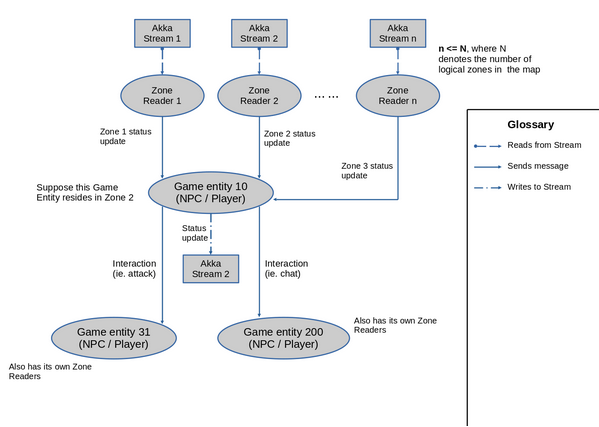
\includegraphics[width=1\textwidth]{../assets/architecture.png}
    \caption{Diagrama de arquitectura propuesta utilizando el modelo de actores y streams}
\end{figure}

\subsection{Backend: servidor distribuido Akka}
\index{Desarrollo}

\subsubsection{Introducción a Akka}

\subsubsection{Arquitectura}

\subsubsection{Diagramas}

\subsubsection{Mensajes de Kafka}

Como fue explicado anteriormente, para la comunicación de eventos utilizamos Kafka mediante actores especializados para la
lectura y escritura llamados \textbf{Consumidores} y \textbf{Productores} respectivamente. Dichos actores operan sobre
mensajes que contienen información relacionada a un evento. Para serializar los mensajes de una forma eficiente usamos
la herramienta Protobuf, explicada en detalle en la sección 8.4.

\subsection{Frontend: cliente Godot}

\noindent \textit{Godot} es un motor para desarrollo de videojuegos, de origen argentino, gratuito y de código abierto. 
Este motor brinda distintas herramientas para desarrollar aplicaciones interactivas, como por ejemplo 
interfaces gráficas, gráficos 2D y 3D, input del usuario con distintos periféricos, control de audio, 
lógica de físicas y colisiones, conectividad a través de la red, entre muchas otras.
Además de permitir desarrollar para múltiples plataformas, permite programar scripts exponiendo una 
API orientada a objetos en los lenguajes C++, C\# e incluso GDScript, un lenguaje propio de Godot. 

\begin{figure}[htbp]
    \centering
    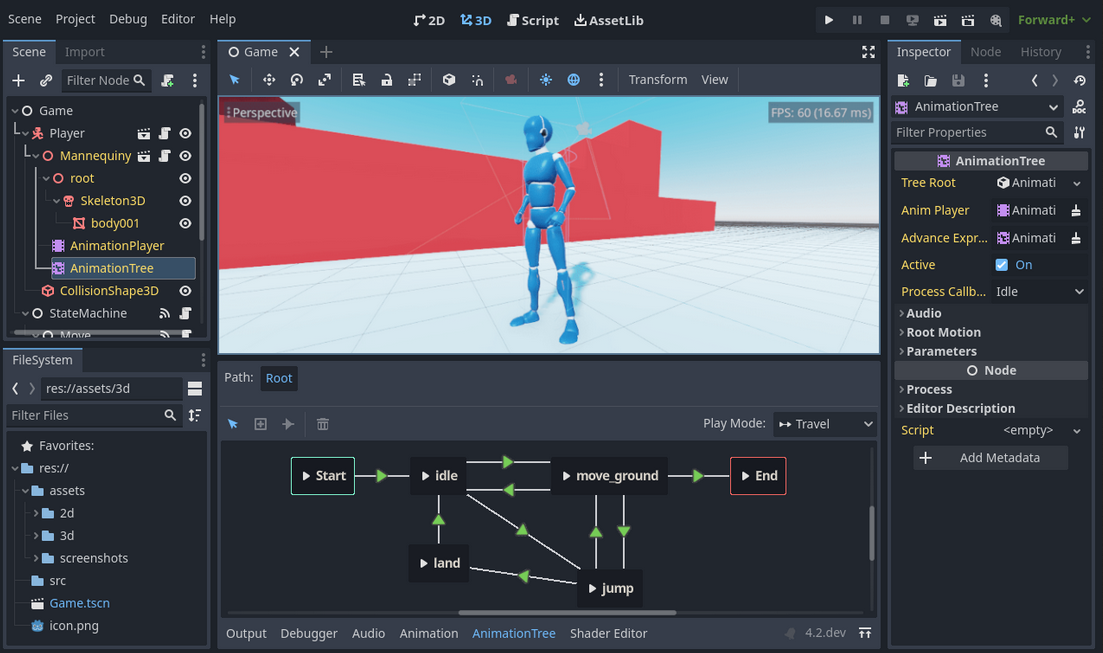
\includegraphics[width=1.0\textwidth]{../assets/godot-engine-showcase.png}
    \caption{Editor de Godot Engine. 
            Source: https://docs.godotengine.org/en/stable/getting\_started/introduction/introduction\_to\_godot.html}
\end{figure}

\textit{GDScript} es un lenguaje de programación de alto nivel y con sintaxis similar a Python. 
El hecho de que sea un lenguaje interpretado tiene la ventaja de que no es necesario volver a compilar 
todo el código cada vez que se hacen modificaciones sobre el mismo.
A partir de la versión 4.0 de Godot, GDScript ofrece soporte opcional de tipado estático, el cual puede
mejorar la performance en runtime y aumenta la eficiencia del código.

\begin{figure}[htbp]
    \centering
    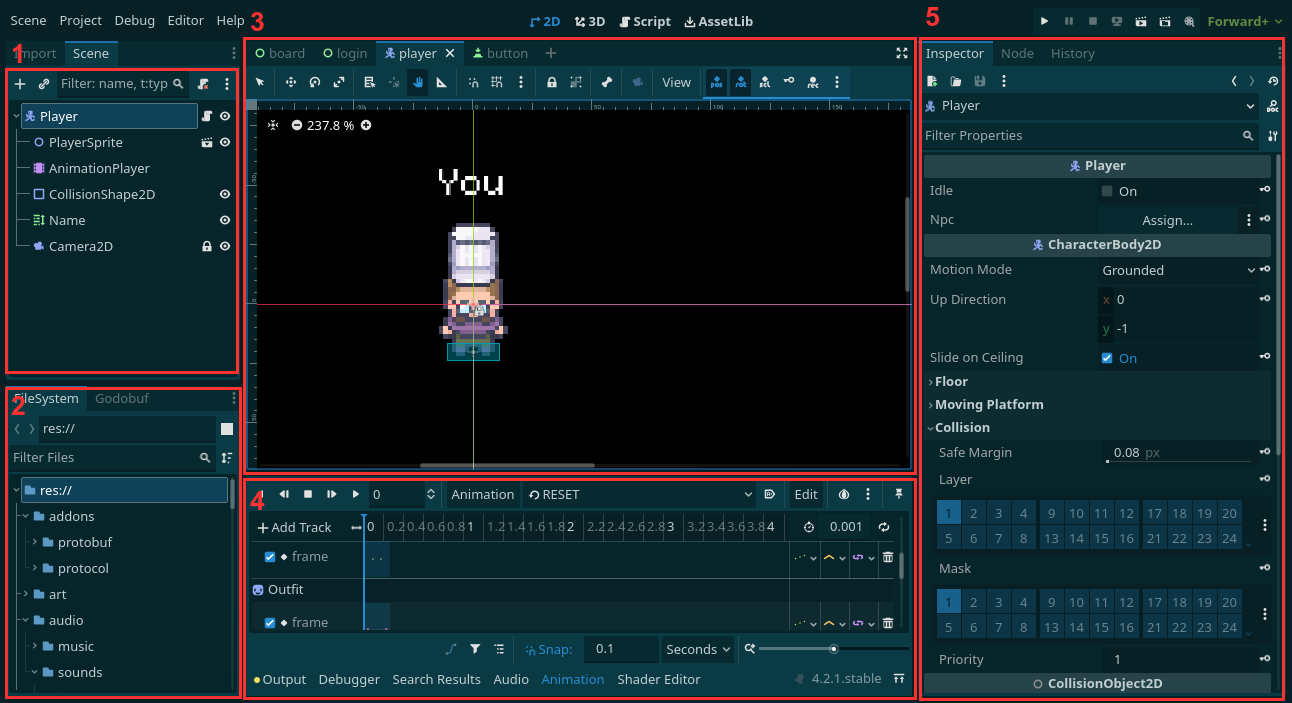
\includegraphics[width=1.0\textwidth]{../assets/godot-editor.png}
    \caption{Editor de código de Godot.}
\end{figure}

El motor ofrece una amplia colección de Nodos, que son los componentes básicos que se utilizan para 
construir Escenas. A su vez, estas escenas pueden ser sub-nodos de otras escenas. Los Nodos pueden ser desde un 
simple botón (\textbf{Button}) hasta un cuerpo tridimensional con lógica de físicas y colisiones 
(\textbf{PhysicsBody3D}) e incluso un \textbf{AnimationPlayer} que se encarga de manejar animaciones, 
es decir, una secuencia de imágenes o \textit{Sprites}.

Estos nodos no solamente son modificables y configurables como se desee, sino que además se les puede 
añadir un script, extendiendo y personalizando su comportamiento como sea necesario.

\begin{figure}[htbp]
    \centering
    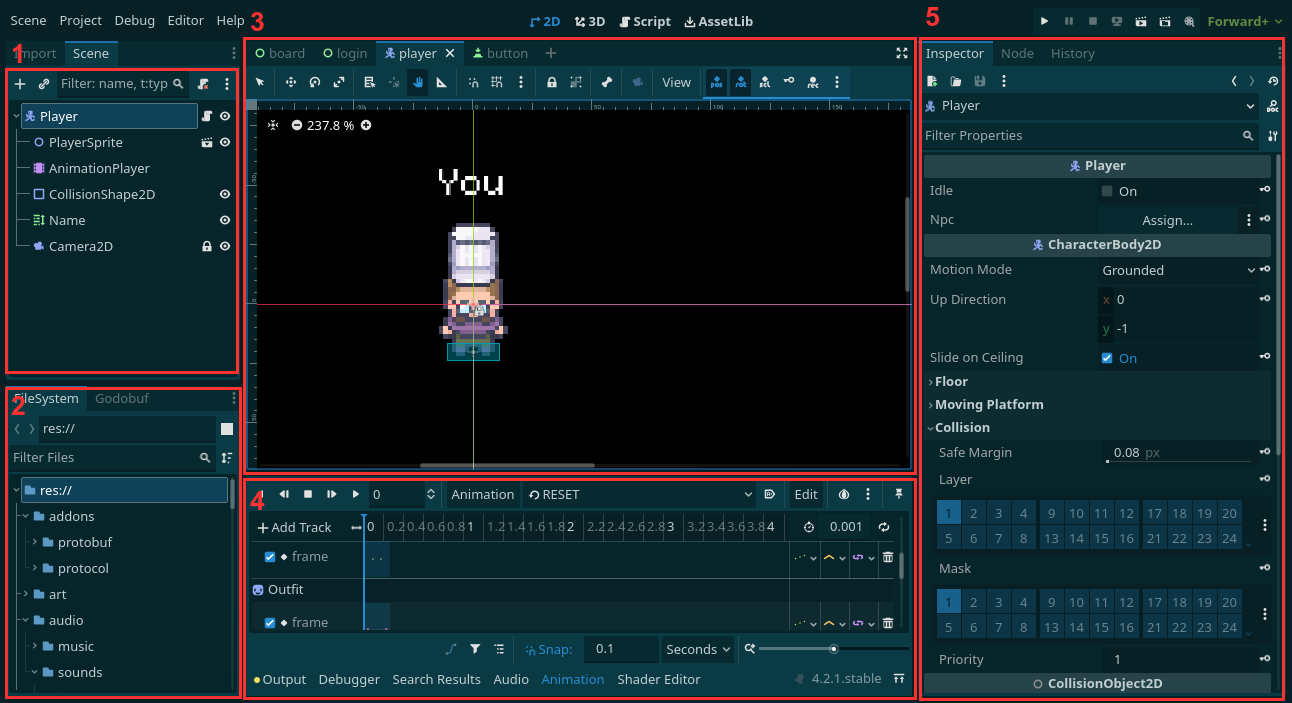
\includegraphics[width=1.0\textwidth]{../assets/godot-editor.png}
    \caption{Interfaz gráfica del editor de Godot. Los componentes enumerados son el árbol de nodos (1),
            el explorador de archivos (2), el editor de la escena (3), el panel de animaciones (4) y el
            inspector del nodo seleccionado (5).}
\end{figure}

Otro feature importante de Godot es el uso de señales (\textit{signals}) para comunicar eventos entre nodos.
Un Nodo cualquiera o una Escena personalizada pueden emitir \textit{signals} con un nombre específico 
(incluso con parámetros) para que otros Nodos o Escenas se suscriban a dicha señal. Al suscribirse, los 
Nodos receptores definen un handler (comúnmente nombrado \textit{\_on\_node\_signal\_name}) para manejar 
la señal recibida. De esta forma se pueden crear escenas compuestas de múltiples Nodos distintos, con 
comportamiento más complejo, pero sin acoplar todos los nodos que necesiten comunicarse entre sí.

\begin{figure}[htbp]
    \centering
    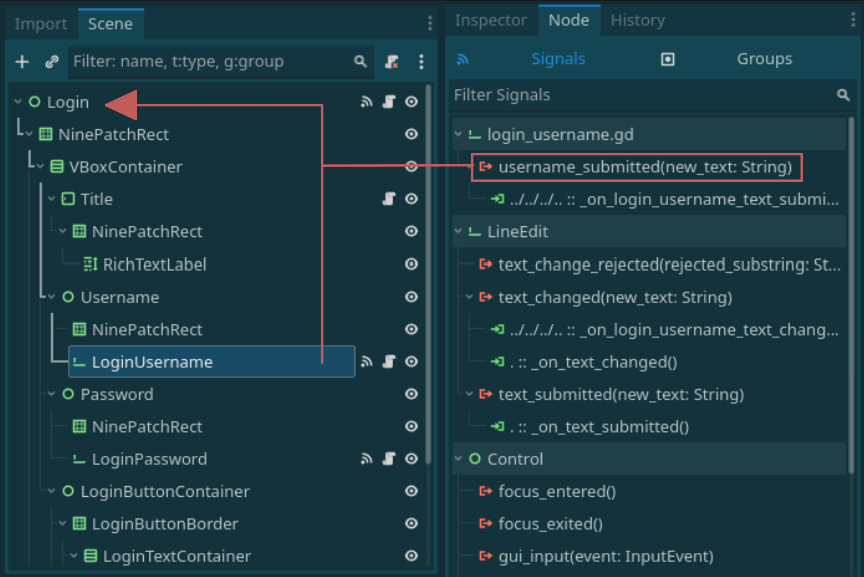
\includegraphics[width=1.0\textwidth]{../assets/godot-signals.png}
    \caption{Ejemplo de conexión de una signal. Cuando el nodo LoginUsername emite la signal
            username\_submitted, el nodo Login la recive en su función \_on\_login\_username\_text\_submitted}
\end{figure}

\begin{figure}[htbp]
    \centering
    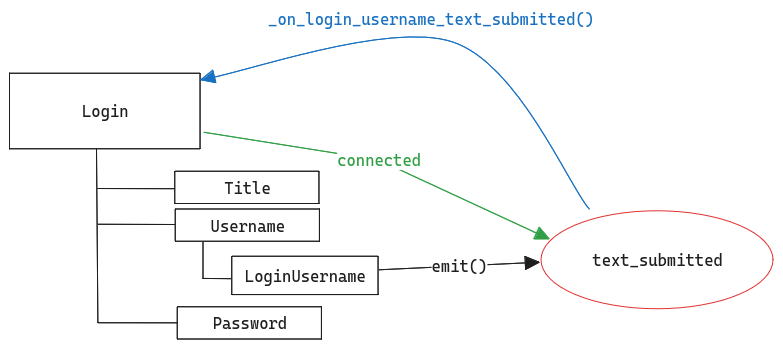
\includegraphics[width=1.0\textwidth]{../assets/godot-signals-diagram.png}
    \caption{Diagrama del flujo de emisión de una signal. Primero se define la señal text\_submitted
            en el nodo LoginUsername y se la conecta al nodo Login (que es padre de LoginUsername).
            Al emitirse esta señal, Login la escucha y entonces ejecuta su función handler
            \_on\_login\_username\_text\_submitted}
\end{figure}

La filosofía del diseño de Godot es construir escenas reutilizables usando nodos. A estas escenas y 
nodos se les puede agregar comportamiento con \textit{scripts}. Con la composición y jerarquía de los Nodos, 
se puede construir una lógica de juego que es clara y fácil de entender.
Es por estas características de cohesión, simplicidad y eficiencia en el diseño de Godot, así
como también el tipo de herramientas que provee que optamos por usar este motor para el desarrollo del
frontend del proyecto en lugar de crear módulos de autoría propia con un lenguaje de más bajo nivel, 
como por ejemplo C o C++.

\subsubsection{Estructura de proyecto}

\noindent Para este proyecto, definimos una Escena \textbf{Main} donde se instancian las escenas más importantes 
del juego, necesarias para el funcionamiento del mismo, como el Menú Principal (\textbf{MainMenu}),
las pantallas de login (\textbf{Login} y \textbf{Register}) y los nodos necesarios para la conexión 
con el Servidor (\textbf{ServerConsumer}, \textbf{ServerProducer}, entre otros).
Los niveles propiamente dichos no se instancian al iniciar el juego, sino una vez que el jugador 
se haya conectado al servidor y luego a medida que se mueve por las distintas zonas del juego.
De esta forma, encapsulamos todas las escenas activas en un mismo lugar y 
no desperdiciamos recursos instanciandolas a la vez, solo se instancian las escenas que
se van a usar.

Además hacemos uso de los \textbf{Autoloads} de Godot, que funcionan igual que el patrón \textbf{Singleton}. 
Se definieron ciertas Escenas y scripts que son necesarios en un scope global como Autoloads.
Por ejemplo, para el manejo, carga y borrado de escenas, hacemos uso de un \textbf{SceneManager}, 
que es un script Autoload que permite transicionar entre niveles dentro del juego. En general, 
se implementaron Singletons de tipo \textit{Manager} para acceder a distintos comportamientos y 
configuraciones globales (información del jugador, cambio de escenas, control del audio, entre otros).

\begin{figure}[htbp]
    \centering
    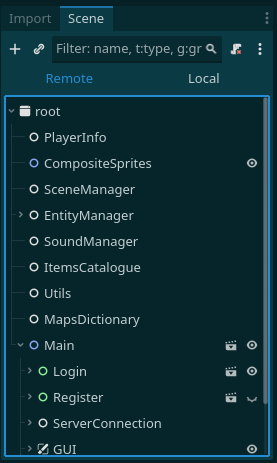
\includegraphics[width=0.4\textwidth]{../assets/godot-scene-tree-1.png}
    \caption{Arbol de nodos (Scene Tree) en la pantalla principal del juego}
\end{figure}

\begin{figure}[htbp]
    \centering
    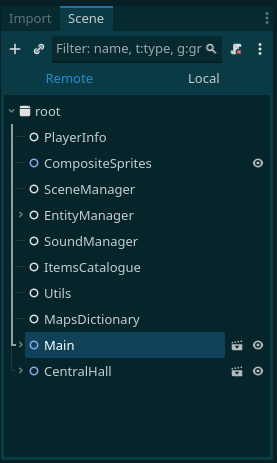
\includegraphics[width=0.4\textwidth]{../assets/godot-scene-tree-2.png}
    \caption{Arbol de nodos cuando el jugador está en un nivel del juego}
\end{figure}


\subsubsection{Comunicación con el servidor}

\noindent Al comienzo del proyecto, un posible limitante de usar Godot eran las herramientas que podía ofrecer 
el motor para la conectividad con el servidor, ya sea UDP, TCP o incluso HTTP. 
Para nuestro beneficio, Godot provee distintas APIs para conectividad que cumplen los requisitos
de los protocolos antes mencionados. En nuestro caso, decidimos usar el protocolo TCP por sus características:
\begin{itemize}
    \item Handshake con el Servidor
    \item Conexión mantenida con el Servidor
    \item Garantía de recepción de todos los paquetes enviados
    \item \textit{Flow Control}
\end{itemize}

Luego, definimos nuestras propias clases \textit{wrapper} para establecer la conexión al servidor y el 
manejo de mensajes. 

Para la recepción implementamos un \textbf{ServerConsumer} que se encarga de recibir los paquetes 
del Servidor, parsea el mensaje completo (ver sección Protocol buffers) y según qué mensaje recibió, 
invoca al \textit{handler} correspondiente para actualizar el estado del juego del lado del Cliente.
Este \textbf{ServerConsumer} se ejecuta en un thread aparte, para no bloquear el thread principal mientras
esperamos recibir un mensaje. Sin embargo, luego de parsear un mensaje recibido, el \textit{handler}
correspondiente se ejecuta en el thread principal.

Es análogo el envío de mensajes en el sentido desde el Cliente hacia el Servidor: algún input de un 
usuario dispara una \textit{signal} que el \textbf{ServerProducer} recibe, este se encarga de crear 
el mensaje correspondiente con los parámetros correctos, lo serializa y envía los paquetes de bytes 
al Servidor a través de la conexión TCP.

\subsection{Comunicación entre cliente y servidor}


\subsubsection{Lógica del juego: movimiento y colisiones}
\noindent Otro de nuestros problemas iniciales fue decidir cómo implementaríamos el movimiento del 
jugador. Al tratarse de un juego online, lo ideal era que la lógica fuera mayormente implementada del 
lado del servidor y así garantizar que los jugadores no pudieran realizar movimientos prohibidos, como 
ir a zonas que no estuvieran permitidas u obtener algún tipo de ventaja. Con este acercamiento del 
problema, Godot no debería hacer más que enviar los inputs de la dirección a la que se desea mover el 
jugador del jugador, y dejar que el 
servidor se encargara de verificar que se tratase de un input válido, calcular el efecto de este 
input en la posición y enviar a Godot la nueva dirección para que se viera reflejada en el juego.

Este acercamiento sirvió en un inicio donde el juego era un prototipo donde no teníamos definidos 
mapas con un perímetro definido, sin embargo empezaron a verse las faltas en esta solución cuando 
se comenzó a implementar las colisiones del jugador con los mapas y los objetos dentro de sus límites.

Se decidió ceder la mayor parte de la lógica del movimiento a Godot debido a que este provee 
su propio sistema de colisiones, aprovechando las herramientas que provee sin reinventar un sistema 
colisiones. Este acercamiento nos hacía renunciar a que el input fuera 
verificado con cada movimiento, pero facilitaba de forma significativa la implementación del 
movimiento y las colisiones. Debido a que nuestro juego no muestra ninguna ventaja competitiva 
en la modificación del movimiento del jugador, decidimos perder parte de las verificaciones en 
favor a la facilidad de desarrollo provista por Godot.

% algoritmos de colisiones son resolubles en el backend, era reiventar la rueda, ya tenemos godot <3
% y no sabíamos cómo iba a ir el tema de performance.

\subsubsection{Juego de cartas: Truco}
\noindent A modo de muestra del tipo de funcionalidades que se pueden desarrollar en conjunto de 
Godot y el modelo de actores, hemos implementado el juego de cartas \textbf{Truco}, específicamente 
en su versión argentina.

Al igual que con el movimiento del jugador y las colisiones, debimos decidir qué 
responsabilidades recaerían tanto para el frontend como para el backend. En la sección 
sobre el movimiento del jugador, concluímos que no existía una importante necesidad de 
validar cada movimiento del jugador, pero el caso de un minijuego como el Truco es distinto. 
En el movimiento, que los demás jugadores vean a otro jugador en una posición incorrecta es 
corregible, momentáneo e insignificante, pero en el Truco, que un jugador presencie una acción 
incorrecta es inaceptable debido a que cada acción realizada por un jugador afecta el flujo del juego.

Para poder mantener la coherencia y la integridad de una partida de Truco, se decidió dejar 
la responsabilidad del manejo de flujo y las verificaciones al backend, mientras que el 
frontend tiene la responsabilidad de mostrarle al jugador todo lo que el backend dicte, 
como por ejemplo las cartas en su mano, las jugadas de su adversario y los cantos disponibles. 
El frontend también posee la responsabilidad de ofrecerle una buena jugabilidad al jugador, 
por lo que la interfaz de juego fue diseñada con estas intenciones. Implementamos un método 
de movimiento para jugar las cartas denominado “drag and drop” para que el jugador pueda 
arrastrar las cartas en caso de que desee jugarlas o volver a colocarla en la mano con tan 
solo volver a arrastrarla a su zona original y una interfaz que muestre los cantos disponibles; 
un cartel que aparezca para avisarle al jugador que su oponente realizó un canto y que luego 
desaparezca, indicadores de a qué jugador le corresponde realizar una jugada, entre otras cosas.


\subsection{Protocol buffers}

\noindent Tanto la comunicación por TCP entre Cliente y Servidor, como el envío de eventos con Kafka
requirió que definamos un protocolo de mensajes propio. Además de definir dicho protocolo, necesitamos
que sea rápido y eficiente, para mantener al mínimo la latencia entre mensajes y poder manejar
una alta cantidad de mensajes.
Es por esto que decidimos usar \textit{Protocol buffers} (o \textit{protobufs}), un mecanismo desarrollado
por Google para serializar datos estructurados, ajeno completamente a cualquier lenguaje.
El propósito es definir los mensajes del protocolo una sola vez y reutilizarlos tanto en el Cliente como el Servidor.
Otra de las razones por la cual elegimos usar esta herramienta fue que cuenta con soporte tanto para Scala como para Godot.
Esto nos permitió que, una vez definidos los mensajes en sus correspondientes archivos \textit{.proto}, podamos usarlos
directamente en el código como si fueran objetos y la herramienta se encarga automáticamente de la serializacion, ya sea para enviar
el mensaje por TCP o para encolarlo en Kafka.

\noindent El formato de todos los mensajes consiste en una sección de metadata y otra sección que contiene el contenido del mensaje específico,
más dos campos de 4 bytes cada uno que indican el largo (en bytes) total del mensaje y el de la sección de metadata.
El campo de metadata contiene a su vez dos campos: uno con el largo del contenido y otro con el tipo del mensaje.
\begin{figure}[htbp]
    \centering
    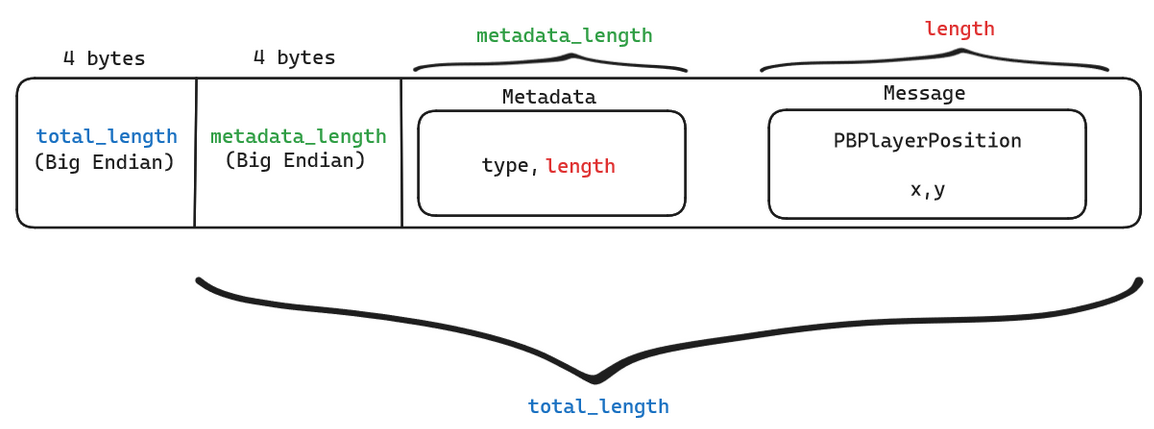
\includegraphics[width=1.0\textwidth]{../assets/protobuf.png}
\end{figure}

Para enviar un mensaje, el flujo es el siguiente: Creamos un objeto que tenga el formato correspondiente a alguno de los
mensajes definidos. Luego, lo serializamos con el método correspondiente de protobuf (según estemos en Scala o Godot) y
calculamos la cantidad de bytes que contiene. Armamos tambien el objeto de metadata, incluyendo el largo calculado y el tipo
del contenido y lo serializamos. Luego, calculamos su largo y calculamos el largo total del mensaje y lo incluimos al principio
del mensaje.

Para leer un mensaje recibido el flujo es el contrario: Leemos los primeros 4 bytes que nos indican el largo
total del mensaje. Luego, leemos los 4 bytes con la cantidad de bytes de metadata. Con esta información, podemos leer
el campo de metadata, que a su vez nos indica el tipo y el largo del contenido. Finalmente, al saber el tipo del contenido, lo
deserializamos para luego poder manejarlo correctamente.

Los mensajes de contenido están definidos en archivos \textit{.proto}. Por ejemplo, veamos el siguiente
mensaje que definimos para el movimiento de un usuario:
\begin{verbatim}
    message PBPlayerVelocity {
        required float x = 1;
        required float y = 2;
    }

    message PBPlayerPosition {
        required float x = 1;
        required float y = 2;
    }

    message PBPlayerMovement {
        required PBPlayerVelocity velocity = 1;
        required PBPlayerPosition position = 2;
    }
\end{verbatim}

El mensaje que el Cliente enviará es \textbf{PBPlayerMovement}, que incluye otros dos mensajes:
\textbf{PBPlayerVelocity} y \textbf{PBPlayerPosition}, ambos vectores bidimensionales representados
por sus coordenadas en \textbf{x} e \textbf{y}. De esta forma cuando el usuario controla y mueve a
su personaje, el Cliente se lo comunica al Servidor creando una instancia de \textbf{PBPlayerMovement}
con los valores correspondientes, serializandolo y finalmente enviándolo.

La totalidad de los mensajes que definimos en nuestro protocolo está en el Anexo \ref{apendix:protobuf}